\documentclass[xetex,mathserif,serif]{beamer}
\usepackage{polyglossia}
\setdefaultlanguage[babelshorthands=true]{russian}
\usepackage{minted}
\usepackage{tabu}

\useoutertheme{infolines}

\usepackage{fontspec}
\setmainfont{FreeSans}
\newfontfamily{\russianfonttt}{FreeSans}

\definecolor{links}{HTML}{2A1B81}
\hypersetup{colorlinks,linkcolor=,urlcolor=links}

\tabulinesep=0.7mm

\newcommand{\attribution}[1] {
	\vspace{-5mm}\begin{flushright}\begin{scriptsize}\textcolor{gray}{\textcopyright\, #1}\end{scriptsize}\end{flushright}
}

\title{Практика по рисованию диаграмм}
\author[Юрий Литвинов]{Юрий Литвинов \newline \textcolor{gray}{\small\texttt{yurii.litvinov@gmail.com}}}

\date{26.02.2020г}

\begin{document}
	
	\frame{\titlepage}

	\begin{frame}
		\frametitle{Практика по рисованию диаграмм}
		\begin{itemize}
			\item Практикуемся в рисовании диаграмм UML
			\item Делать на паре, к концу второй пары сдать на HwProj
			\begin{itemize}
				\item Можно показывать и задавать вопросы
			\end{itemize}
			\item По одному баллу максимум за каждую задачу
			\item Задач много, вряд ли успеете все
			\begin{itemize}
				\item Можно выбирать и делать в любом порядке
			\end{itemize}
			\item \url{https://www.uml-diagrams.org/}
		\end{itemize}
	\end{frame}

	\section{Диаграммы активностей}

	\begin{frame}
		\frametitle{Диаграммы активностей}
		\framesubtitle{Activity diagrams}
		\begin{center}
			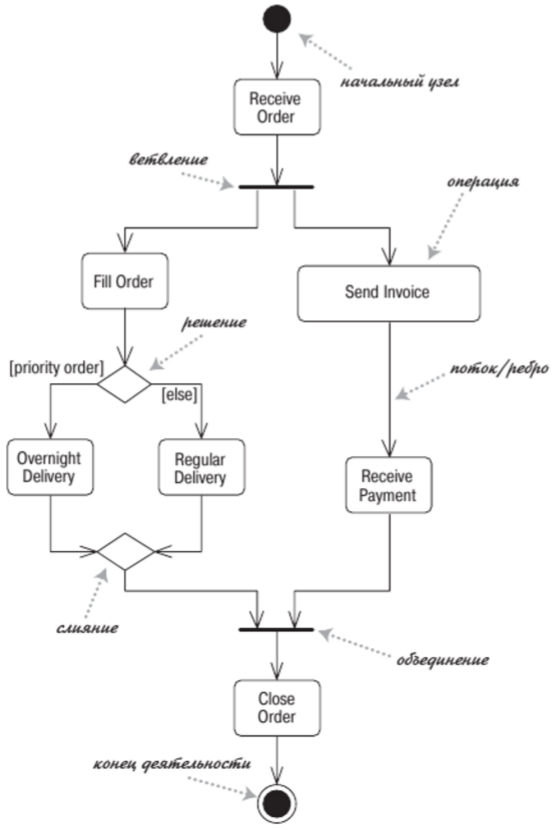
\includegraphics[width=0.415\textwidth]{activityDiagram.png}
		\end{center}
	\end{frame}

	\begin{frame}
		\frametitle{Диаграммы активностей, разделы}
		\framesubtitle{Swimlanes}
		\begin{center}
			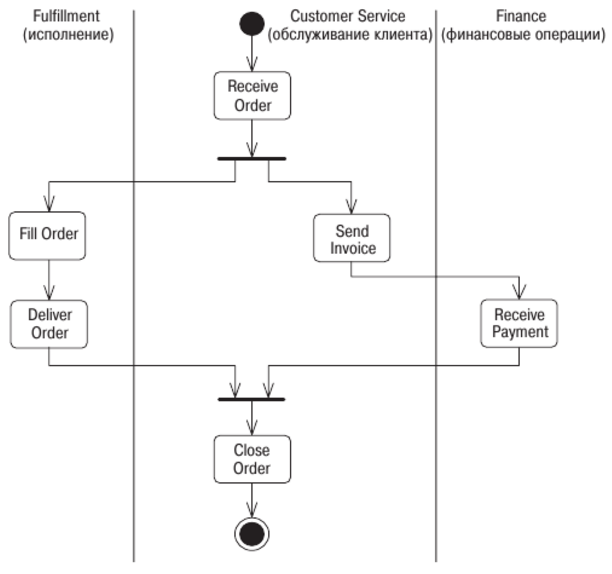
\includegraphics[width=0.55\textwidth]{activitySwimlanes.png}
		\end{center}
	\end{frame}

	\begin{frame}
		\frametitle{Задача 1}
		Нарисовать диаграмму активностей, моделирующую бизнес-процесс проведения ``промежуточной аттестации'' с точки зрения как студента, так и учебного отдела
		\begin{itemize}
			\item Допуски по практикам
			\item Экзамены
			\item Результаты --- отчисление, перевод в следующий семестр
			\item Использовать разделы для представления разных заинтересованных сторон
		\end{itemize}
	\end{frame}

	\section{Диаграммы последовательностей}

	\begin{frame}
		\frametitle{Диаграммы последовательностей}
		\framesubtitle{Sequence diagrams}
		\begin{center}
			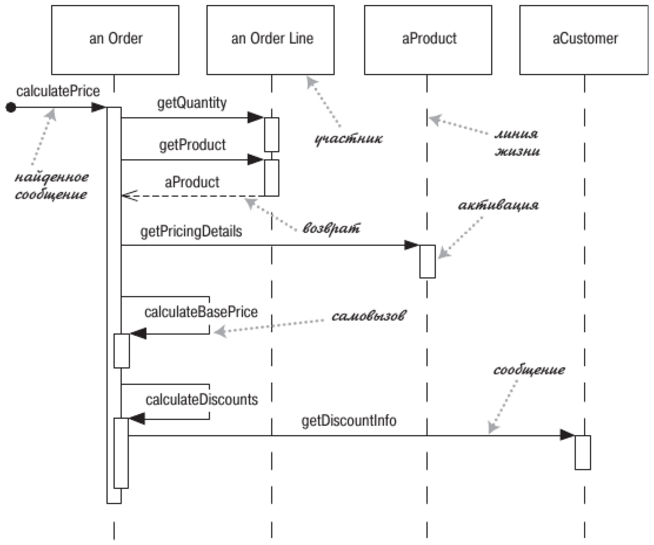
\includegraphics[width=0.6\textwidth]{sequenceDiagram.png}
		\end{center}
	\end{frame}

	\begin{frame}
		\frametitle{Диаграммы последовательностей, создание и удаление объектов}
		\begin{center}
			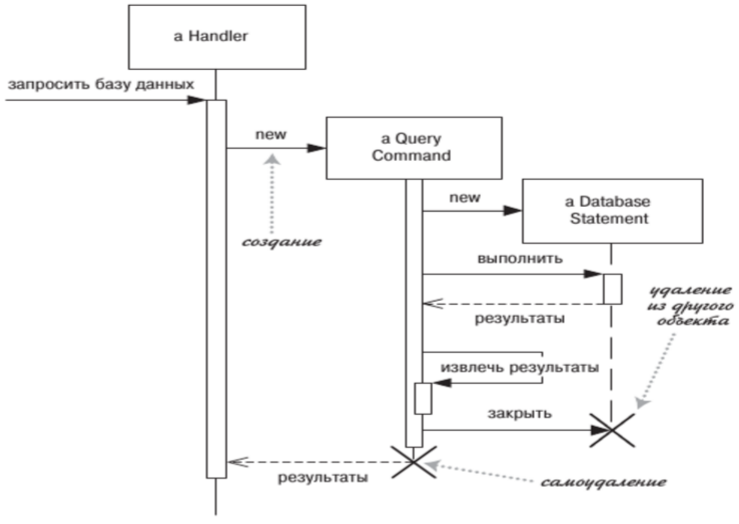
\includegraphics[width=0.65\textwidth]{sequenceLifeCycle.png}
		\end{center}
	\end{frame}

	\begin{frame}
		\frametitle{Диаграммы последовательностей, фреймы}
		\begin{center}
			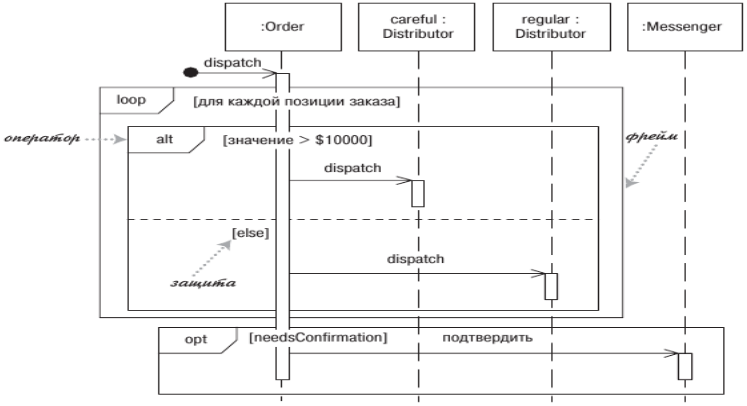
\includegraphics[width=0.8\textwidth]{sequenceFrames.png}
		\end{center}
	\end{frame}

	\begin{frame}
		\frametitle{Задача 2}
		Нарисовать диаграмму последовательностей --- типичный сценарий взаимодействия пользователя и HwProj при посылке решения
		\begin{itemize}
			\item Начиная с авторизации и до окончания взаимодействия
			\item HwProj умеет общаться с GitHub-ом, чтобы проверить статус пуллреквеста
		\end{itemize}
	\end{frame}

	\section{Коммуникационные диаграммы}

	\begin{frame}
		\frametitle{Коммуникационные диаграммы}
		\begin{columns}
			\begin{column}{0.5\textwidth}
				\begin{itemize}
					\item Применяются для визуализации взаимодействия между объектами
					\begin{itemize}
						\item Более легковесный аналог диаграмм последовательностей
						\item Тоже отображают один сценарий взаимодействия
					\end{itemize}
				\end{itemize}
			\end{column}
			\begin{column}{0.5\textwidth}
				\begin{center}
					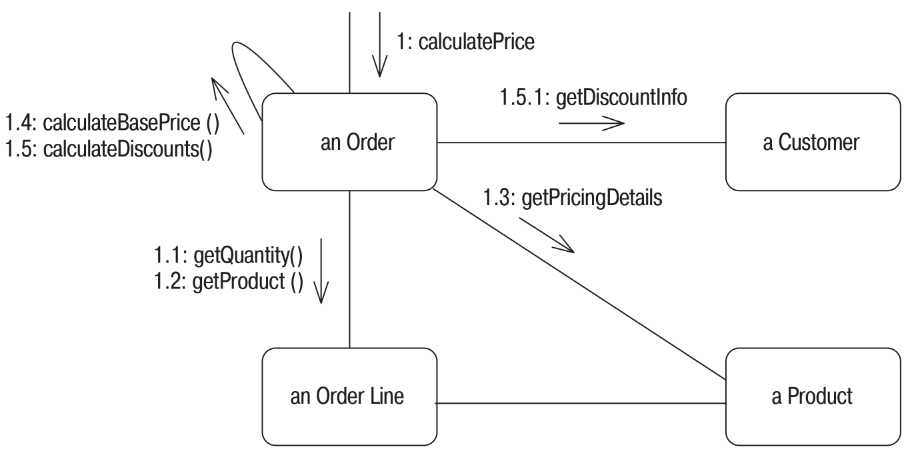
\includegraphics[width=\textwidth]{communicationDiagram.png}
					\attribution{М. Фаулер, UML. Основы}
				\end{center}
			\end{column}
		\end{columns}
	\end{frame}

	\begin{frame}
		\frametitle{Задача 3}
		Нарисовать то же самое в виде коммуникационной диаграммы
	\end{frame}

	\section{Диаграммы развёртывания}

	\begin{frame}
		\frametitle{Диаграмма развёртывания UML}
		\begin{columns}
			\begin{column}{0.5\textwidth}
				\begin{itemize}
					\item Показывает отображение компонентов и физических артефактов на реальные (или виртуальные) устройства
					\item Бывает полезна на начальных этапах проектирования, даже до диаграмм компонентов
				\end{itemize}
			\end{column}
			\begin{column}{0.5\textwidth}
				\begin{center}
					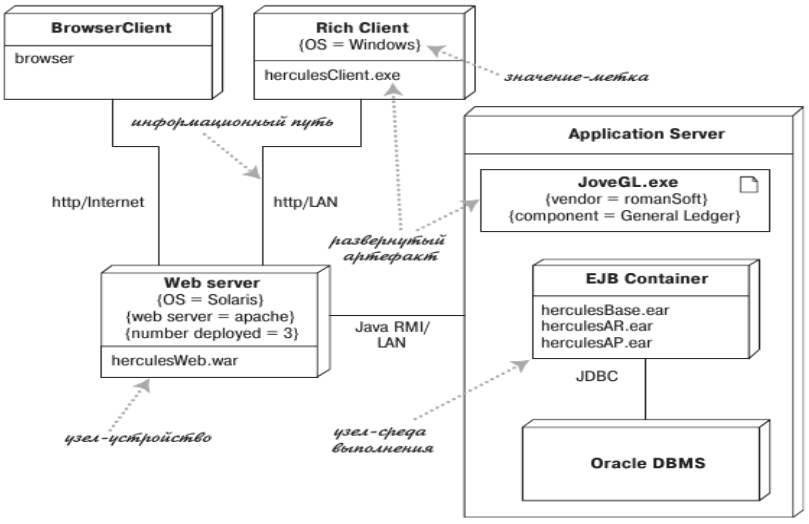
\includegraphics[width=\textwidth]{deploymentDiagram.png}
					\attribution{М. Фаулер, UML. Основы}
				\end{center}
			\end{column}
		\end{columns}
	\end{frame}

	\begin{frame}
		\frametitle{Задача 4}
		Нарисовать диаграмму развёртывания для приложения, описанного в RFP про автомобильный завод
		\begin{itemize}
			\item \url{https://goo.gl/MiyH8c}
		\end{itemize}
	\end{frame}

	\section{Диаграммы конечных автоматов}

	\begin{frame}
		\frametitle{Диаграммы конечных автоматов}
		\framesubtitle{Диаграммы состояний}
		\begin{columns}
			\begin{column}{0.4\textwidth}
				\begin{itemize}
					\item Состояния объекта как часть жизненного цикла
					\item Моделирование реактивных объектов
					\begin{itemize}
						\item Например, сетевое соединение
					\end{itemize}
				\end{itemize}
			\end{column}
			\begin{column}{0.6\textwidth}
				\begin{center}
					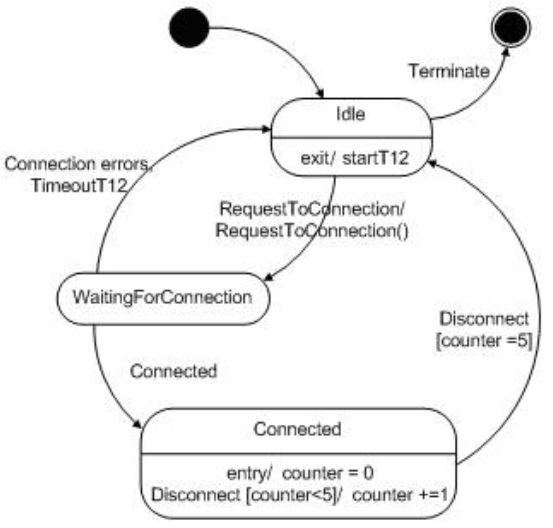
\includegraphics[width=0.7\textwidth]{stateTransitionExample.png}
				\end{center}
			\end{column}
		\end{columns}
	\end{frame}

	\begin{frame}
		\frametitle{Диаграммы конечных автоматов, синтаксис}
		\begin{columns}
			\begin{column}{0.5\textwidth}
				\begin{itemize}
					\item Состояние
					\begin{itemize}
						\item entry activity
						\item exit activity
						\item do activity
						\item внутренний переход
					\end{itemize}
					\item Событие
					\item Переход
					\begin{itemize}
						\item имя события (список параметров) [сторожевое условие] выражение действия
					\end{itemize}
				\end{itemize}
			\end{column}
			\begin{column}{0.5\textwidth}
				\begin{center}
					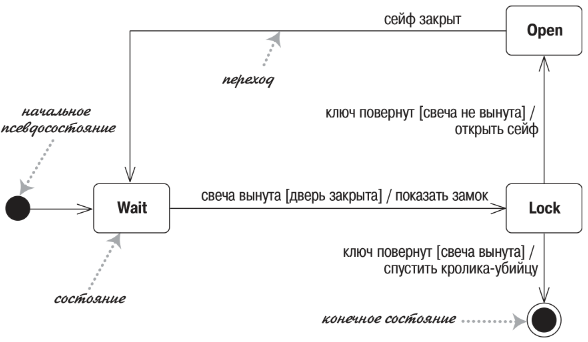
\includegraphics[width=\textwidth]{stateTransitionSyntax.png}
					\attribution{М. Фаулер, UML. Основы}
				\end{center}
			\end{column}
		\end{columns}
	\end{frame}

	\begin{frame}
		\frametitle{Задача 5}
		Нарисовать диаграмму конечных автоматов, описывающую поведение микроволновки
	\end{frame}

	\section{Временные диаграммы}

	\begin{frame}
		\frametitle{Временные диаграммы}
		\begin{columns}
			\begin{column}{0.5\textwidth}
				\begin{center}
					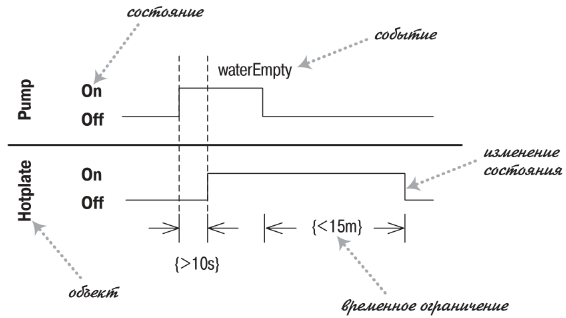
\includegraphics[width=0.9\textwidth]{timingDiagrams.png}
				\end{center}
			\end{column}
			\begin{column}{0.5\textwidth}
				\begin{center}
					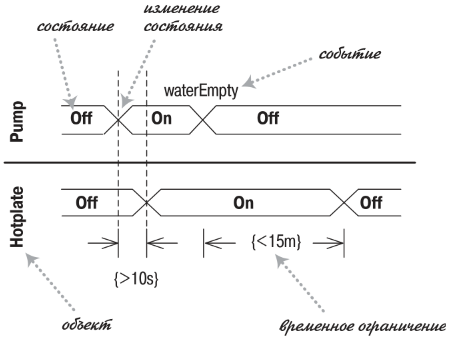
\includegraphics[width=0.8\textwidth]{timingDiagramsAlternate.png}
					\attribution{М. Фаулер, UML. Основы}
				\end{center}
			\end{column}
		\end{columns}
	\end{frame}

	\begin{frame}
		\frametitle{Задача 6}
		Нарисовать временную диаграмму любого сценария работы микроволновки
		\begin{itemize}
			\item В VP это может быть не совсем тривиально: \url{https://www.visual-paradigm.com/support/documents/vpuserguide/94/2586/6715_drawingtimin.html}
		\end{itemize}
	\end{frame}

\end{document}
